\chapter{Análisis y arquitectura}
\label{chap:analisis_arquitectura}

\lettrine{E}{n} este capítulo se detallan los requisitos del sistema y la arquitectura tecnológica seleccionada para la implementación del Datamart y el cuadro de mando. Es importante destacar que todo el proyecto se ha diseñado y desarrollado utilizando exclusivamente tecnologías \textbf{Open Source} (código abierto). Esta decisión estratégica garantiza que cualquier centro educativo, sea público o privado, pueda adoptar y desplegar esta solución sin incurrir en costes de licenciamiento de software comercial.

\section{Requisitos del sistema}

Para lograr el objetivo de detectar de forma temprana el riesgo de abandono escolar y la brecha digital, el sistema debe cumplir con los siguientes requisitos funcionales y no funcionales:

\begin{itemize}
    \item \textbf{RF1 - Extracción y Transformación:} El sistema debe ser capaz de extraer datos en bruto del sistema transaccional (PostgreSQL), limpiarlos y aplicar reglas de negocio para calcular índices de riesgo socioeconómico y académico.
    \item \textbf{RF2 - Modelo Dimensional:} Los datos deben estructurarse en un Data Warehouse bajo un modelo de estrella para facilitar consultas analíticas ultrarrápidas y cruces demográficos.
    \item \textbf{RF3 - Visualización y Alertas:} Se debe proveer una interfaz web (Dashboard) que muestre de forma intuitiva qué centros educativos o cohortes geográficas presentan un riesgo alto de vulnerabilidad sistémica y fracaso escolar.
    \item \textbf{RNF1 - Modularidad y Escalabilidad:} La arquitectura debe estar dividida en microservicios independientes, facilitando su despliegue y mantenimiento.
    \item \textbf{RNF2 - Tecnologías Libres:} Obligatoriedad de utilizar herramientas Open Source en todas las capas del proyecto.
\end{itemize}

\section{Análisis del sistema transaccional origen}

Para comprender la necesidad de construir un Data Warehouse y diseñar los flujos ETL, es fundamental analizar previamente la estructura de la base de datos origen. En este proyecto se ha simulado una base de datos transaccional (OLTP) en PostgreSQL que replica el sistema de gestión académica y administrativa estándar de los centros educativos.

Este sistema está altamente normalizado para garantizar la integridad referencial y evitar la redundancia de datos en las operaciones diarias (altas de matrículas, registro de calificaciones, encuestas familiares). El modelo relacional consta de 14 tablas principales interconectadas (ver Figura \ref{fig:diagrama_er_origen} y Figura \ref{fig:modelo_relacional_origen}), agrupadas en los siguientes dominios lógicos:

\begin{itemize}
    \item \textbf{Dominio Académico:} Tablas \textit{CICLO\-\_EDUCATIVO}, \textit{ESPECIALIDAD}, \textit{CURSO} y \textit{ASIGNATURA}. Definen el catálogo formativo del sistema.
    \item \textbf{Dominio de Matriculación y Evaluación:} Tablas \textit{CENTRO}, \textit{ADMISION}, \textit{MATRICULA}, \textit{ASIGNATURA\-\_MATRICULA} y la entidad débil \textit{LINEA\-\_EXPEDIENTE}, que almacena el histórico de calificaciones por evaluación.
    \item \textbf{Dominio del Alumnado y Diversidad:} Tablas \textit{ESTUDIANTE}, \textit{ADAPTACION\-\_CURRICULAR} y \textit{ADAPTACION\-\_ASIGNATURA}, registrando los expedientes y las medidas de apoyo educativo.
    \item \textbf{Dominio Socioeconómico:} Tablas \textit{RESPONSABLE\-\_LEGAL} y \textit{ENCUESTA}. Contienen el histórico de ingresos, acceso a internet y nivel educativo de los progenitores; datos vitales para calcular posteriormente el riesgo socioeconómico.
\end{itemize}

Dada la alta fragmentación de la información (por ejemplo, para relacionar las calificaciones de un estudiante con el nivel de renta de sus tutores es necesario cruzar simultáneamente las tablas \textit{LINEA\-\_EXPEDIENTE}, \textit{ASIGNATURA\-\_MATRICULA}, \textit{MATRICULA}, \textit{ESTUDIANTE}, \textit{RESPONSABLE\-\_LEGAL} y \textit{ENCUESTA}), ejecutar algoritmos analíticos directamente sobre este esquema penalizaría severamente el rendimiento del sistema en producción. Esta limitación inherente a los sistemas OLTP justifica plenamente el diseño dimensional del Datamart.

% ==========================================
% DIAGRAMAS DEL ALUMNO
% ==========================================

\begin{figure}[htbp]
    \centering
    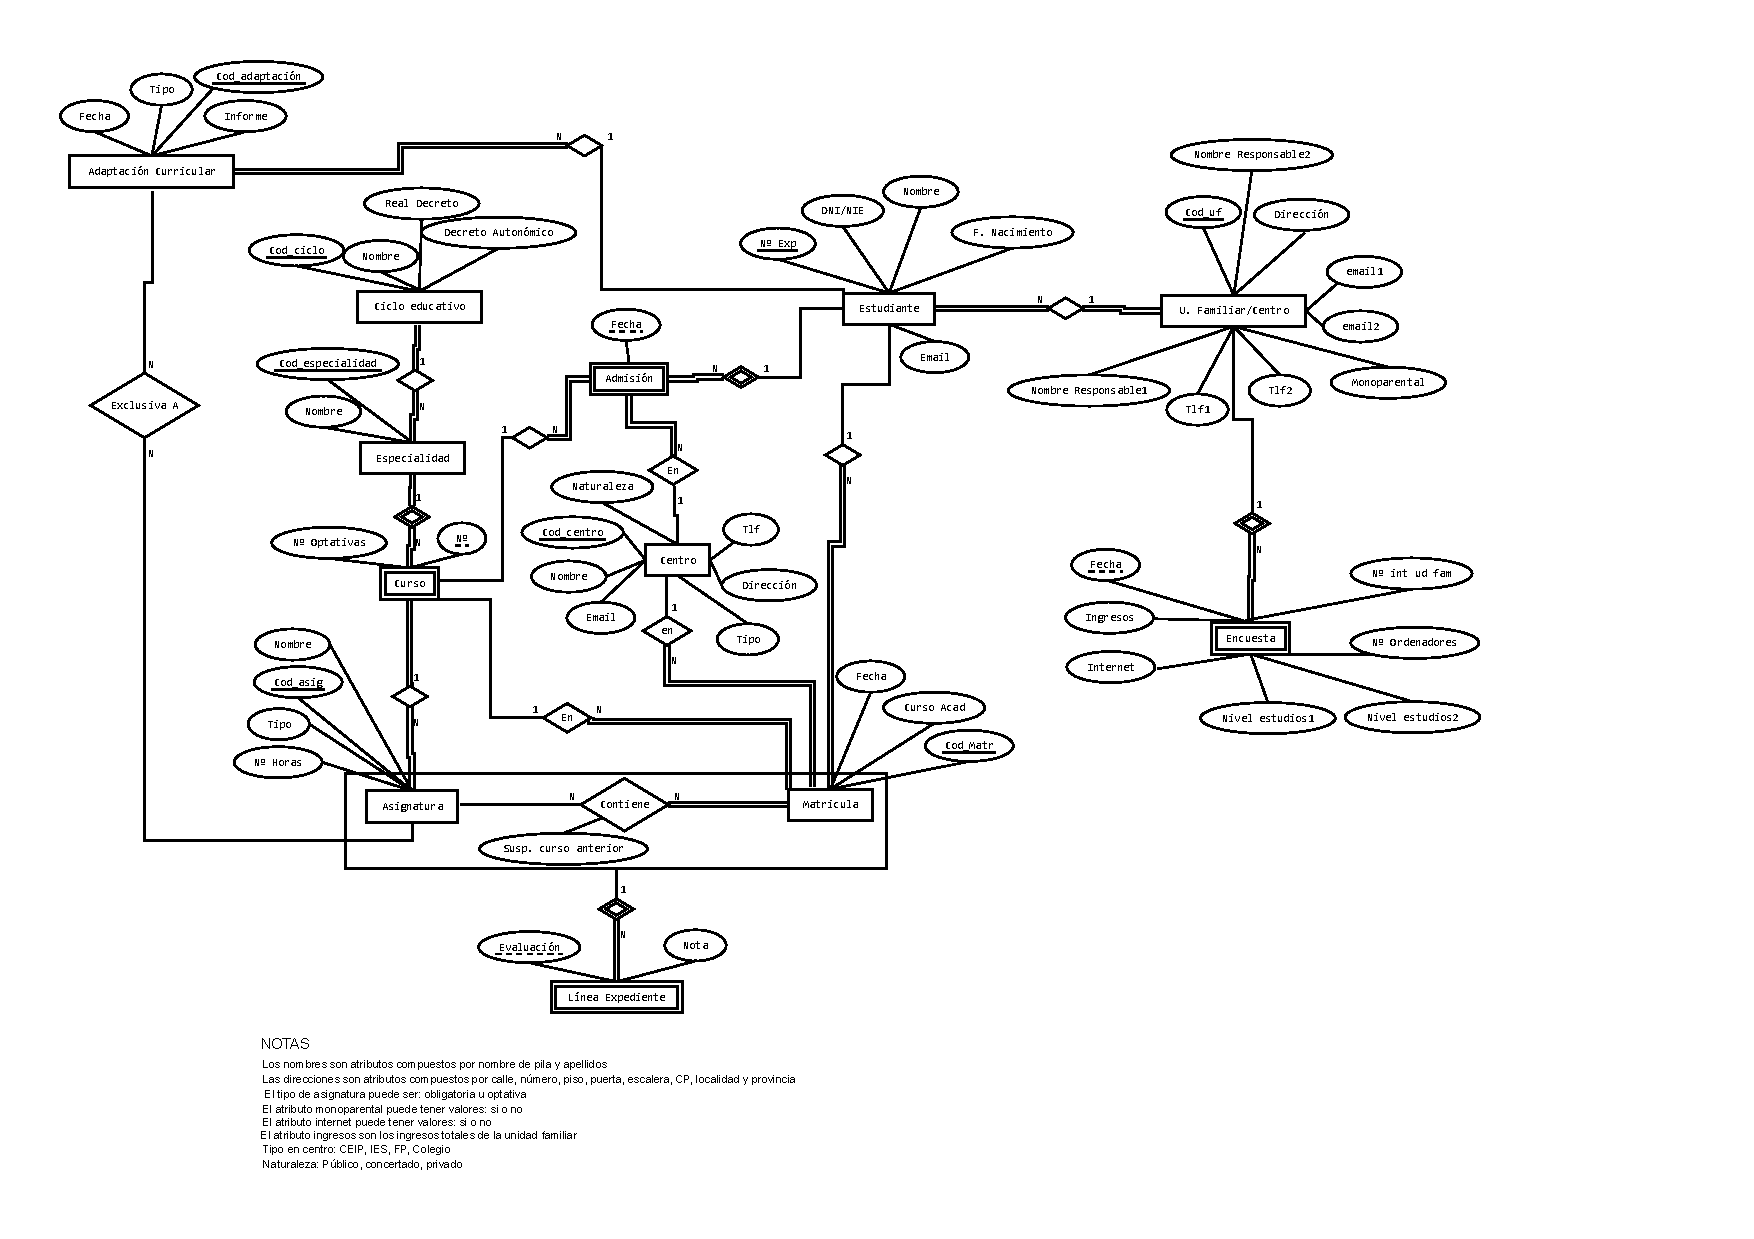
\includegraphics[width=1\textwidth]{imaxes/modelo_er_source.pdf}
    \caption{Modelo Entidad-Relación (ER) de la base de datos transaccional origen.}
    \label{fig:diagrama_er_origen}
\end{figure}

\begin{figure}[htbp]
    \centering
    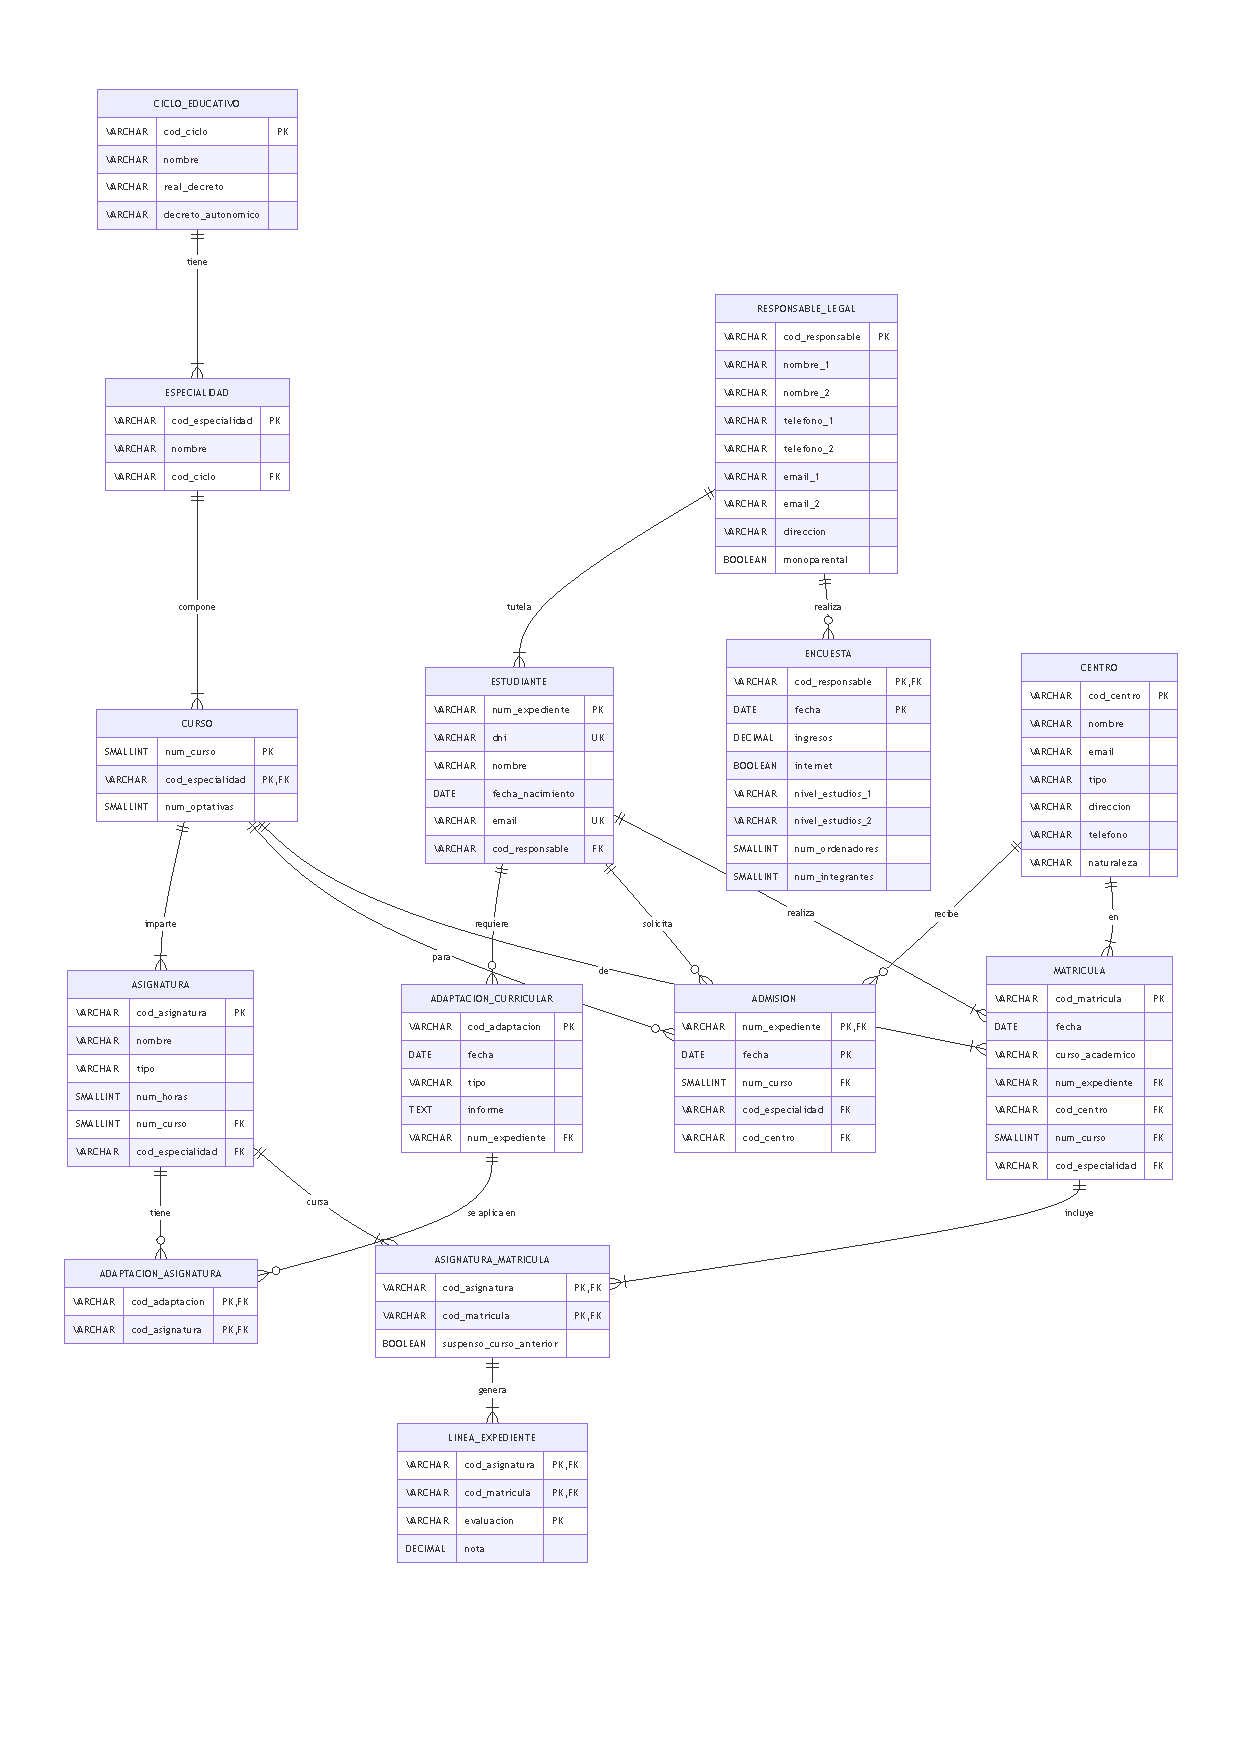
\includegraphics[width=1\textwidth]{imaxes/relacional_source.pdf}
    \caption{Esquema Relacional de origen.}
    \label{fig:modelo_relacional_origen}
\end{figure}

\section{Arquitectura tecnológica basada en Docker}

Para cumplir con el requisito de modularidad, la arquitectura del proyecto se ha construido bajo el paradigma de contenedores utilizando \textbf{Docker} \cite{Docker_Docs}. Esto permite aislar cada componente del sistema en su propio entorno, asegurando que funcionen de manera predecible independientemente del servidor donde se desplieguen.

El ecosistema está compuesto por seis contenedores principales orquestados mediante \textit{docker-compose}:

\begin{enumerate}
    \item \textbf{Origen de Datos Transaccional (PostgreSQL)} \cite{PostgreSQL_Docs}: Simula la base de datos operativa (\textit{source}) de los centros educativos. Contiene tablas normalizadas con los expedientes, matrículas, notas y encuestas familiares en tiempo real.
    \item \textbf{Data Warehouse Analítico (PostgreSQL)}: Actúa como el repositorio central de BI (\textit{dwh}). Almacena los datos estructurados en un modelo dimensional (esquema en estrella) optimizado para lectura y agregación, conteniendo el historial acumulado.
    \item \textbf{Orquestador ETL (Apache Hop Web)}: Contenedor que ejecuta los flujos de transformación (\textit{pipelines}). Se encarga de conectarse al Origen de Datos, extraer la información, calcular las métricas de riesgo (socioeconómico y de abandono) y cargar el resultado en el Data Warehouse.
    \item \textbf{Servidor Backend RESTful (FastAPI)} \cite{FastAPI_Docs}: Construido en Python, este contenedor expone una API segura que se conecta al Data Warehouse, realiza las consultas analíticas pesadas mediante \textit{SQLAlchemy} y sirve los resultados en formato JSON al cliente.
    \item \textbf{Aplicación Cliente Dashboard (React/Vite)} \cite{React_Docs}: Interfaz gráfica web moderna donde los gestores de la administración visualizan los datos. Utiliza \textit{Recharts} para los gráficos y sigue una estética visual basada en \textit{Glassmorphism}.
    \item \textbf{Servidor Web y Proxy Inverso (Nginx)}: Se encarga de servir la aplicación React compilada y de enrutar las peticiones de red hacia la API del Backend, asegurando un único punto de entrada seguro para la aplicación.
\end{enumerate}

Esta separación clara entre la base de datos transaccional (OLTP) y el almacén analítico (OLAP) garantiza que las complejas consultas del Dashboard no penalicen el rendimiento de las operaciones diarias del colegio.

\subsection{Justificación del paradigma de contenedores}

Aunque el diseño de una arquitectura distribuida conlleva una mayor carga de razonamiento inicial respecto a una solución monolítica, esta decisión aporta un enorme valor añadido al proyecto por tres motivos fundamentales:

\begin{itemize}
    \item \textbf{Aislamiento y Reproducibilidad:} Cada contenedor empaqueta sus propias dependencias (por ejemplo, librerías concretas de Python para FastAPI o módulos de Node para React). Esto elimina el clásico problema de \textit{"funciona en mi máquina"} y garantiza que el comportamiento del software sea idéntico en desarrollo, pruebas y producción.
    \item \textbf{Despliegue Universal (\textit{One-Click Deployment}):} Al estar orientado a centros educativos (instituciones que frecuentemente carecen de departamentos de IT especializados o presupuestos para infraestructuras complejas), la orquestación con \textit{docker-compose} permite levantar toda la plataforma (bases de datos, ETL, API y web) con un único comando. Esto facilita enormemente su transferencia tecnológica y adopción real.
    \item \textbf{Topología de Red y Seguridad:} Docker permite crear redes virtuales cerradas (\textit{Docker Networks}). De esta forma, bases de datos críticas como el Data Warehouse y los flujos de transformación de Apache Hop quedan totalmente invisibles desde el exterior. Solamente el proxy inverso (Nginx) expone los puertos estrictamente necesarios, añadiendo una capa de seguridad pasiva esencial cuando se tratan datos académicos y demográficos de menores.
\end{itemize}
